% !TeX spellcheck = ru_RU
% !TEX root = vkr.tex

\section{Описание решения}

Перед тем как подробно рассмотреть реализацию, приведём схематичный алгоритм работы системы:
\begin{enumerate}
    \item Получение веб-страницы: определение необходимости JS-рендеринга с помощью \texttt{is\_dynamic\_site(url, timeout)} (см.\cite{PatilWebScraping2021, Smith2022}) и загрузка содержимого (статический запрос \cite{RequestsDocumentation} или рендеринг через Selenium \cite{SeleniumDocumentation}).
    \item Очистка HTML: выбор стратегии очистки (\texttt{FullCleaningStrategy} или \texttt{LightCleaningStrategy} \cite{Richardson2013, Brown2020}) в зависимости от режима (\emph{Structuring} или \emph{Codegen}).
    \item Интеграция с LLM: формирование промптов и вызов \texttt{LLMClient} из библиотеки MistralAI \cite{MistralAIDocumentation}, генерация структурированных данных (Structuring) или кода-парсера (Codegen) \cite{Kalyan2023, Li2024}.
    \item Кэширование: сохранение сгенерированных скриптов и/или результатов структурирования в SQLite и ChromaDB \cite{SQLiteDocumentation, ChromaDBDocumentation, Reimers2019} для повторного использования без дополнительных обращений к LLM \cite{Dong2022CacheLLM}.
    \item Выполнение парсера или разбора JSON: если найден кэш, загружается готовый скрипт; иначе выполняется вновь сгенерированный код или парсинг через Structuring, результат возвращается в формате JSON.
    \item Вывод результата пользователю через Gradio, REST-API или веб-frontend \cite{FastAPIDocumentation, GradioDocumentation, Jinja2Documentation}.
\end{enumerate}

В проекте реализованы два основных режима работы с LLM:
\begin{itemize}
    \item \emph{Structuring} — прямая генерация структурированных данных (JSON) из текста страницы \cite{Brown2020}.
    \item \emph{Codegen} — генерация Python-скрипта-парсера, который затем выполняется локально \cite{Dong2022CacheLLM}.
\end{itemize}
Для уменьшения затрат на повторные обращения к LLM внедрён механизм кэширования, использующий как реляционную базу SQLite, так и векторную базу ChromaDB для семантического поиска близких запросов \cite{Reimers2019, ChromaDBDocumentation}.

\subsection{Получение и предварительная обработка веб-страницы}
\label{subsec:solution1}

Чтобы определить, требуется ли JavaScript-рендеринг, используется функция \texttt{is\_dynamic\_site(url, timeout)} (файл \texttt{autoparse/tools/fetchers/dynamic\_detector.py}). Она возвращает \texttt{True}, если хотя бы один из следующих критериев выполнен:
\begin{enumerate}
    \item Статический HTTP-запрос (\texttt{fetch\_static\_html(url, timeout)}) завершился ошибкой \cite{RequestsDocumentation}.
    \item После парсинга через BeautifulSoup длина текста внутри тега \texttt{<body>} менее 300 символов \cite{Richardson2013}.
    \item В документе более 10 тегов \texttt{<script>}.
    \item У любого тега \texttt{<script>} атрибут \texttt{type} равен \texttt{"module"} или \texttt{"application/json"}.
    \item В атрибуте \texttt{src} тега \texttt{<script>} встречаются подстроки \texttt{"react", "angular", "vue", "ember", "svelte", "next", "nuxt"} \cite{W3Techs2024}.
    \item Содержимое inline-скриптов содержит \texttt{"window.\_\_"} или \texttt{"hydrate("}.
    \item В DOM присутствуют атрибуты гидрации: \texttt{data-reactroot}, \texttt{data-reactid}, \texttt{data-vue} или \texttt{data-server-rendered}.
    \item В документе найден элемент с \texttt{id} равным одному из \texttt{"app", "root", "main", "container", "next", "nuxt"}.
\end{enumerate}

В классе \texttt{Parser} (\texttt{autoparse/parser.py}) метод \texttt{parse\_url(url, \dots)} действует так:
\begin{itemize}
    \item Если \texttt{dynamic=True} или \texttt{is\_dynamic\_site(url)} возвращает \texttt{True}, вызывается рендеринг через Selenium (Headless Chrome) \cite{SeleniumDocumentation}.
    \item Иначе применяется статический HTTP-запрос через \texttt{requests} \cite{RequestsDocumentation}.
\end{itemize}
Далее полученный HTML передаётся на этап очистки (см. раздел~\ref{subsec:solution2}).

\subsection{Стратегии очистки HTML-разметки}
\label{subsec:solution2}

Для подготовки HTML к работе с LLM определены две стратегии (интерфейс \texttt{CleaningStrategy} в \texttt{autoparse/strategies/cleaning.py}):

\paragraph{FullCleaningStrategy.}
Полностью удаляет все HTML-теги и возвращает «чистый» текст. Применяется в режиме \emph{Structuring}, когда модель должна «прочитать» текст страницы и сформировать JSON-структуру \cite{Brown2020}. Алгоритм:
\begin{itemize}
    \item Удаление тегов \texttt{<script>}, \texttt{<style>} и комментариев.
    \item Сбор оставшегося текста через метод \texttt{BeautifulSoup.get\_text()} \cite{BeautifulSoupDocumentation}.
\end{itemize}

\paragraph{LightCleaningStrategy.}
Сохраняет базовую структуру HTML, удаляя лишь шумовые элементы (скрипты, стили, комментарии). Применяется в режиме \emph{Codegen}, когда LLM должно получить «облегчённый» HTML для генерации кода-парсера \cite{Dong2022CacheLLM}. Алгоритм:
\begin{itemize}
    \item Удаление тегов \texttt{<script>} и \texttt{<style>}.
    \item Удаление комментариев.
    \item Возврат оставшегося HTML-содержимого.
\end{itemize}

\paragraph{Диспетчер стратегий.}
Метод \texttt{get\_pipeline(html, mode, code\_cache)} (\texttt{autoparse/dispatcher.py}) возвращает пару «стратегия очистки + стратегия парсинга»:
\begin{itemize}
    \item \texttt{mode == "structuring"}: \texttt{FullCleaningStrategy} и \texttt{StructuringParsingStrategy}.
    \item \texttt{mode == "codegen"}: \texttt{LightCleaningStrategy} и \texttt{CodegenParsingStrategy}.
    \item \texttt{mode == "auto"}: если \texttt{is\_dynamic\_site(url)} → как для \emph{Structuring}, иначе → как для \emph{Codegen}.
\end{itemize}

\subsection{Интеграция с LLM: режимы \emph{Structuring} и \emph{Codegen}}
\label{subsec:solution3}

Работа с LLM реализована в папке \texttt{autoparse/tools/llm}. Ниже приведены текстовые описания основных компонентов и алгоритмов.

\subsubsection{Клиент LLM: \texttt{LLMClient}}
\label{sssec:llmclient}

Класс \texttt{LLMClient} (файл \texttt{client.py}) оборачивает SDK MistralAI \cite{MistralAIDocumentation}. Основные моменты:
\begin{itemize}
    \item При инициализации получает API-ключ (\texttt{MISTRAL\_API\_KEY}) и имя модели (\texttt{LLM\_MODEL="mistral-large-latest"}).
    \item Метод \texttt{call\_llm(prompt: str)} отправляет текстовый \texttt{prompt} и возвращает ответ модели в виде строки.
    \item Учитываются ограничения по лимиту токенов через \texttt{tiktoken} \cite{TiktokenDocumentation}.
\end{itemize}

\subsubsection{Режим \emph{Structuring}}
\label{sssec:structuring}

Алгоритм \texttt{StructuringParsingStrategy} выполняется так:
\begin{enumerate}
    \item На вход подаётся «чистый» текст (результат \texttt{FullCleaningStrategy}) и пользовательский запрос (\texttt{user\_query}).
    \item Формируется системный prompt с описанием задачи («Produce JSON…» \cite{Brown2020}) и вставляется сам текст страницы вместе с запросом.
    \item Вызывается \texttt{LLMClient.call\_llm(prompt)}, получаем ответную строку в формате JSON.
    \item Результат обрабатывается через \texttt{json.loads(response\_text)} и возвращается в виде словаря (\texttt{\{"structured\_data": <данные>\}}).
\end{enumerate}

\subsubsection{Режим \emph{Codegen}}
\label{sssec:codegen}

В режиме \emph{Codegen} применяется \texttt{LightCleaningStrategy} и компонент \texttt{hintgen}, который формирует контекст для генерации кода-парсера \cite{Li2024}. Ключевые шаги:
\begin{enumerate}
    \item \textbf{Получение «облегчённого» HTML.} Применяется \texttt{LightCleaningStrategy}, полученный HTML передаётся дальше.
    \item \textbf{Генерация подсказки (\texttt{hintgen}).} Модуль анализирует очищенный HTML и учёт запроса (\texttt{user\_query}), рассчитывает количество токенов через \texttt{tiktoken}, обрезает контекст и формирует Chat-style prompt, включающий:
    \begin{itemize}
        \item Системную инструкцию, объясняющую, какие теги и селекторы искать.
        \item Примеры полей и формат вывода.
        \item Собственно «облегчённый» HTML-фрагмент и запрос пользователя.
    \end{itemize}
    \item \textbf{Поиск в кэше (\texttt{ParserCodeCache.find\_similar}).}
    \begin{itemize}
        \item Формируется уникальный идентификатор \texttt{doc\_id = f"{url}:{user\_query}"}, вычисляется его embedding через модель \texttt{paraphrase-multilingual-MiniLM-L12-v2} \cite{Reimers2019}.
        \item Выполняется запрос к ChromaDB: если косинусное сходство ≥ порога (\texttt{SIMILARITY\_THRESHOLD}), возвращается путь к ранее сгенерированному скрипту из SQLite (кэш считается «попавшим»).
    \end{itemize}
    \item \textbf{Сохранение нового скрипта (если кэш не найден).}
    \begin{itemize}
        \item Вычисляется MD5-хеш от \texttt{url + user\_query}, формируется имя файла \texttt{<hash>.py} в папке \texttt{parsers/}.
        \item Полученный код записывается в этот файл, и в SQLite добавляется новая запись с полями \texttt{url, user\_query, file\_path, timestamp} \cite{SQLiteDocumentation}.
        \item Вычисляется embedding для \texttt{doc\_id} и добавляется в ChromaDB вместе с метаданными (время создания) \cite{ChromaDBDocumentation}.
    \end{itemize}
    \item \textbf{Возврат результата.} Если найден существующий файл, сразу возвращается готовый скрипт; иначе возвращается вновь сгенерированный код в формате JSON вида \texttt{\{"parser\_code": "<python\_code>"\}}.
\end{enumerate}

Таким образом, при наличии «эквивалентного» скрипта пара (\texttt{url}, \texttt{user\_query}) обрабатывается без повторного обращения к LLM, что позволяет снизить затраты и уменьшить задержки \cite{Dong2022CacheLLM, OpenAI2023Costs}.

\subsection{Механизм кэширования и семантического поиска запросов}
\label{subsec:solution4}

Класс \texttt{ParserCodeCache} (\texttt{autoparse/cache/code\_cache.py}) отвечает за хранение и поиск ранее созданных скриптов. Основные моменты:

\paragraph{Инициализация SQLite и ChromaDB.}
При создании \texttt{ParserCodeCache(base\_dir)}:
\begin{itemize}
    \item Создаётся папка \texttt{<base\_dir>/parsers/} для хранения Python-файлов.
    \item Открывается (или создаётся) файл \texttt{<base\_dir>/cache.db}.
    \item Выполняется SQL-команда, создающая таблицу \texttt{code\_cache} с полями \texttt{url}, \texttt{user\_query}, \texttt{file\_path} и \texttt{timestamp}, а также первичным ключом (\texttt{url, user\_query}) \cite{SQLiteDocumentation}.
    \item Инициализируется клиент ChromaDB и embedding-функция (Sentence-BERT), после чего из SQLite загружаются все имеющиеся записи: для каждой записи вычисляется embedding идентификатора \texttt{url:user\_query} и добавляется в коллекцию ChromaDB \cite{Reimers2019, ChromaDBDocumentation}.
\end{itemize}

\paragraph{Поиск «похожих» запросов.}
Метод \texttt{find\_similar(url, user\_query)}:
\begin{enumerate}
    \item Формирует \texttt{doc\_id = f"{url}:{user\_query}"} и вычисляет embedding через модель SentenceTransformer \cite{Reimers2019}.
    \item Делает запрос к коллекции ChromaDB, запрашивая ближайшего соседа. Если его косинусное сходство >= порога (\texttt{SIMILARITY\_THRESHOLD}), извлекает путь к файлу из SQLite и возвращает его; иначе возвращает \texttt{None}.
\end{enumerate}

\paragraph{Сохранение нового скрипта.}
Если \texttt{find\_similar} вернул \texttt{None}, производится:
\begin{enumerate}
    \item Генерация MD5-хеша от строки \texttt{url + user\_query}, формирование имени файла \texttt{<hash>.py} в директории \texttt{parsers/} \cite{Dong2022CacheLLM}.
    \item Запись полученного кода в файл.
    \item Вставка новой записи в таблицу \texttt{code\_cache} (через SQL-команду \texttt{INSERT OR IGNORE} с параметрами \texttt{url, user\_query, file\_path, timestamp}) \cite{SQLiteDocumentation}.
    \item Вычисление embedding для \texttt{doc\_id} и добавление его вместе с путём к файлу в коллекцию ChromaDB \cite{ChromaDBDocumentation}.
\end{enumerate}

\subsection{Пользовательские интерфейсы}
\label{subsec:solution5}

Для удобства взаимодействия с системой созданы три клиента, все они используют единый фасад: функцию \texttt{run\_agent} из модуля \texttt{agent/agent.py}. Ниже приводятся краткие описания.

\subsubsection{Gradio-приложение (Hugging Face Space)}

В файле \texttt{server/HFspace/app.py} настроен интерфейс на основе Gradio, который содержит:
\begin{itemize}
    \item Поле для ввода URL.
    \item Поле для ввода \texttt{user\_query}.
    \item Радиокнопки для выбора режима (\texttt{"auto", "structuring", "codegen"}).
    \item Флаг \texttt{dynamic} для принудительного указания необходимости рендеринга.
    \item Кнопка «Submit», вызывающая функцию вида:
    \begin{quote}
      \texttt{parse\_interface(url, query, mode, dynamic) = run\_agent(\dots)}
    \end{quote}
    Полученный результат (JSON или код-парсер) автоматически отображается через Gradio \cite{GradioDocumentation}.
\end{itemize}

\subsubsection{REST-API на FastAPI}

В файле \texttt{server/api/main.py} реализовано:
\begin{itemize}
    \item Pydantic-модель \texttt{ParseRequest} с полями \texttt{url, user\_query, mode, dynamic}.
    \item POST-эндпоинт \texttt{/parse}, который принимает JSON-запрос, вызывает \texttt{run\_agent} и возвращает ответ в формате JSON.
    \item Для запуска сервера используется команда:
    \begin{quote}
      \texttt{uvicorn server.api.main:app --reload}
    \end{quote}
    \cite{FastAPIDocumentation}.
\end{itemize}

\subsubsection{Веб-frontend (FastAPI + Jinja2 + JavaScript)}

\begin{figure}[h]
    \centering
    \begin{minipage}[b]{0.48\textwidth}
        \centering
        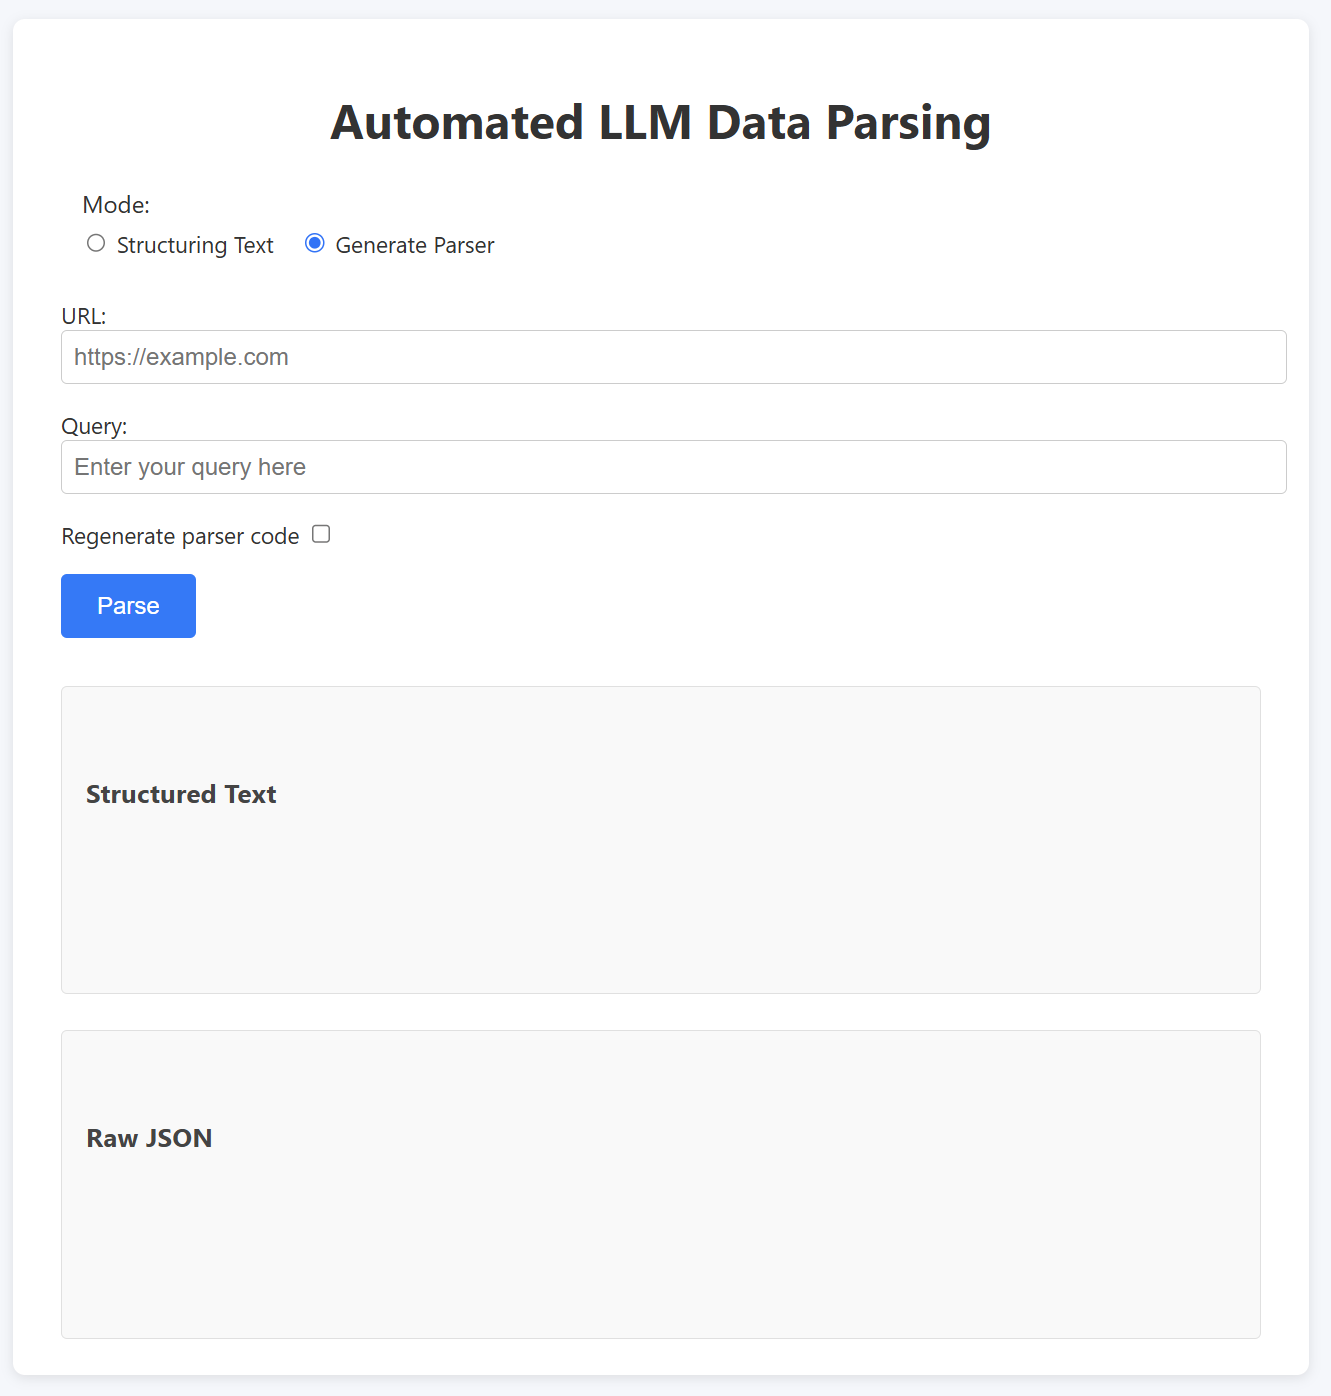
\includegraphics[width=\textwidth]{Include/dashboard_codegen.png}
        \caption{Веб-frontend: режим Codegen}
        \label{fig:dash_codegen}
    \end{minipage}
    \hfill
    \begin{minipage}[b]{0.48\textwidth}
        \centering
        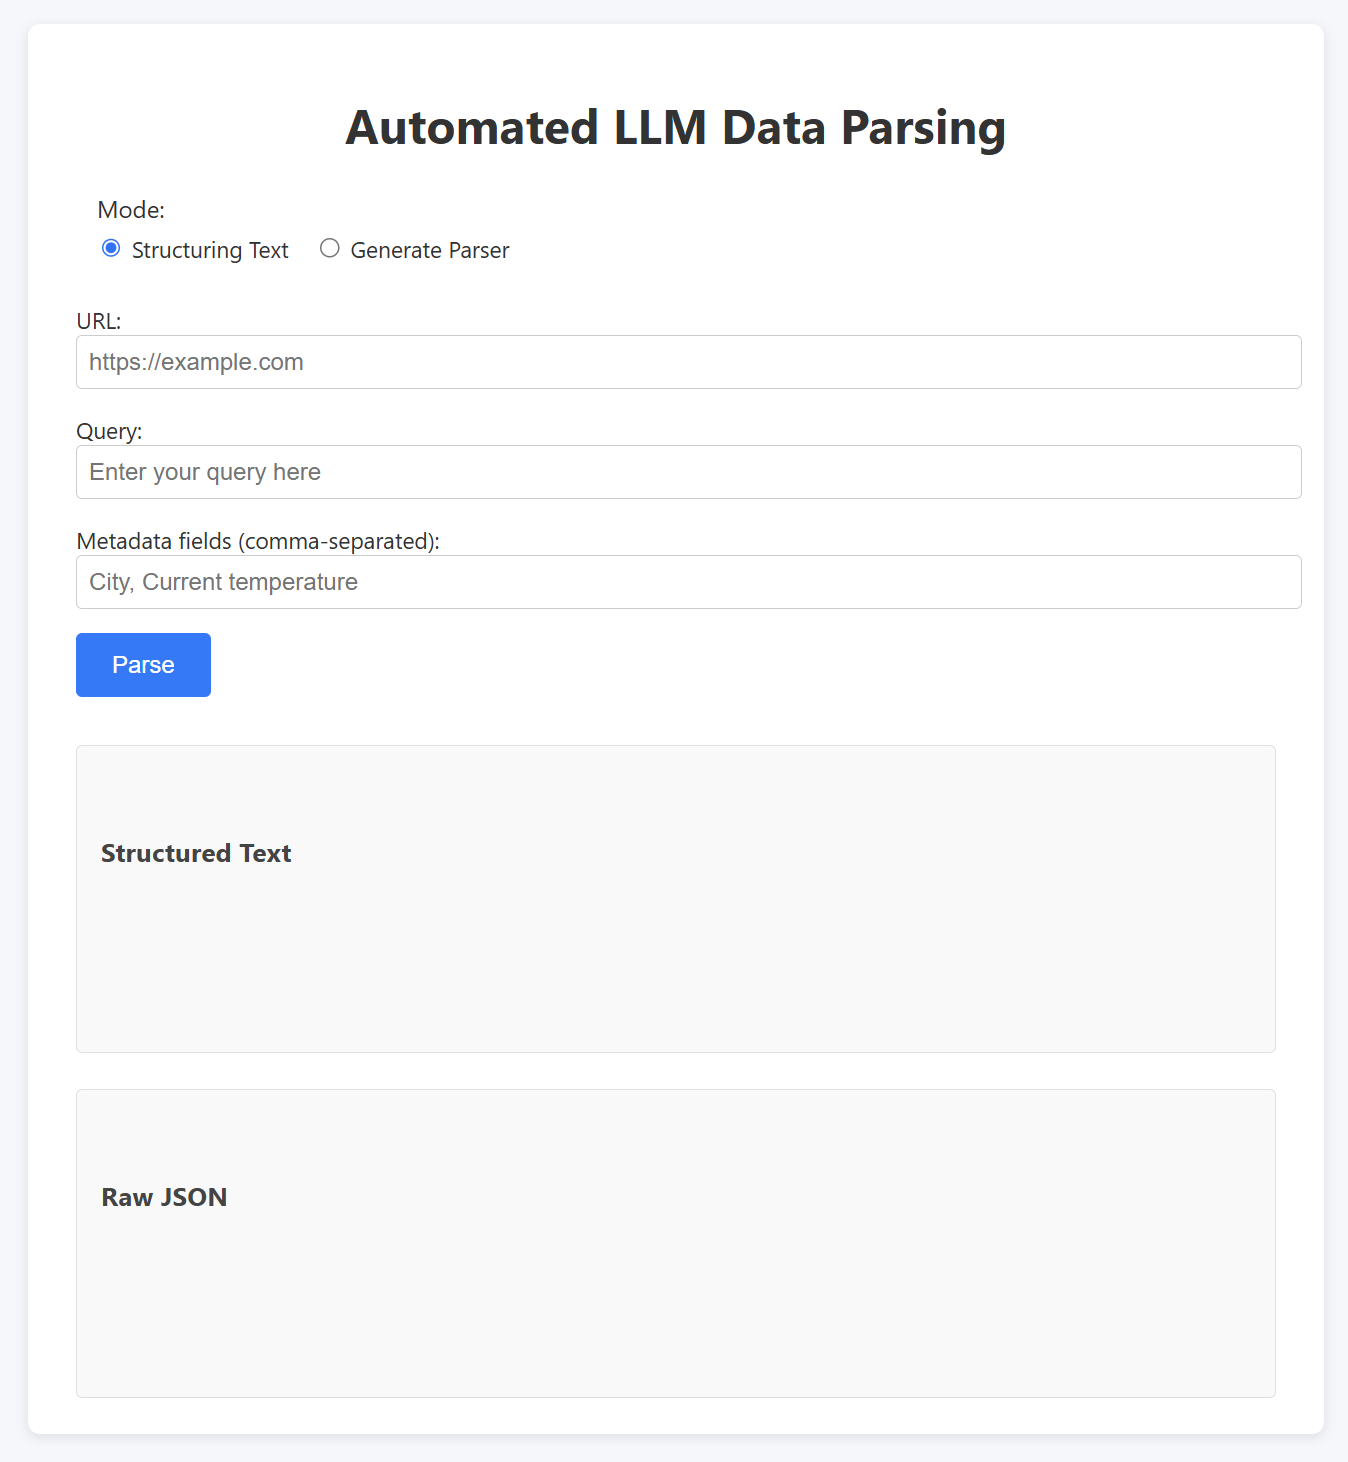
\includegraphics[width=\textwidth]{Include/dashboard_structuring.png}
        \caption{Веб-frontend: режим Structuring}
        \label{fig:dash_structuring}
    \end{minipage}
\end{figure}

В директории \texttt{server/web} настроено:
\begin{itemize}
    \item \texttt{main.py}, который монтирует статические файлы и рендерит шаблон \texttt{index.html}.
    \item В \texttt{templates/index.html} размещена HTML-форма с полями для URL, \texttt{user\_query}, выбора режима и флажка \texttt{dynamic}.
    \item JavaScript-файл \texttt{static/js/app.js} перехватывает отправку формы, выполняет AJAX-запрос к эндпоинту \texttt{/parse\_via\_web} и отображает полученный JSON или код в элементе \texttt{<div id="result">} \cite{Jinja2Documentation}.
\end{itemize}